\documentclass[12pt, a4paper]{article}
\usepackage{amsmath, amssymb, amsthm, mathtools, graphicx, slashed}
\usepackage{subcaption}%Permet d'utiliser subfigure
\usepackage[top=1cm, bottom=1.5cm, left=1cm, right=1cm]{geometry}
\usepackage[compat=1.1.0]{tikz-feynman}
\usepackage{verbatim}
\usepackage{hyperref}
%\tikzfeynmanset{compat=1.1.0}
\title{Devoir de BSM du 28 Juillet 2026 }
\author{RAZAFIMAHERY Faneva Liantsoa\\ 
	\small{Master 2- Physique des Hautes Energies} \\ \small{Université d'Antananarivo}}
\date{\small 3 Août 2026}
\begin{document}
	\maketitle
	\begin{abstract}
		\textit{Dans ce travail, il nous a été demandé de calculer l'amplitude $\mathcal{A}(1^+, 2^+, 3^+, 4^-, 5^-, 6^-)$ en utilisant la technique de récursion BCFW:}\\
		\[\mathcal{A}(1...n)=\sum \mathcal{A}_L \frac{1}{p^2_m} \mathcal{A}_R\]
	\end{abstract}
		\section*{Rappels sur les formules de Parke-Taylor et formules des amplitudes $\mathcal{A}_3$}
		\subsection*{ \normalsize Parke-Taylor }
		\begin{equation}
		\begin{split}
			 \mathcal{A}_{MHV}(1^+,..., i^-,..., j^-,..., n^+)&=\frac{ \langle ij \rangle ^4}{\langle 12 \rangle \langle 23 \rangle...\langle n1 \rangle}\\
			 \mathcal{A}_{anti-MHV}(1^-,..., i^+,..., j^+,..., n^-)&=\frac{ [ij]^4}{[12] [23]...[n1]}\\
		\end{split}
		\end{equation}
		\subsection*{ \normalsize $\mathcal{A}_3$}
		\begin{equation}
			\begin{split}
				\mathcal{A}_3(1^+, 2^-, 3^-)&=\frac{ \langle 23 \rangle ^4}{\langle 12 \rangle \langle 23 \rangle \langle 31 \rangle }\\
				\mathcal{A}_3(1^-,2^+, 3^+)&=\frac{ [23]^4}{[12] [23][31]}\\
			\end{split}
		\end{equation}
		\section{Choix de shift}
		Dans ce qui suit, nous avons utilisé le shift $[61 \rangle$:
		\begin{itemize}
			\item $ \hat{\bar{\lambda}}_6= \bar{\lambda}_6 + z \bar{\lambda}_1 $
			\item $ \hat{\lambda}_1= \lambda_1 - z \lambda_6 $
		\end{itemize}
		
		\section{Diagrammes possibles}
		Avec notre choix de shift et le choix d'hélicité des impulsions $\hat{p}_m$ pour tenir compte du propagateur, nous avons uniquement deux décompositions d'amplitude qui ne valent pas zéros.\\
		Nous les notons $\mathbb{X}$ et $\mathbb{Y}$, voici leurs représentations graphiques:\\
		\begin{figure}[h]
			\centering
			\begin{minipage}[c]{0.10\textwidth}
				\centering
				Pour $\mathbb{X}$
			\end{minipage}
			\begin{minipage}[c]{0.75\textwidth}	
				\centering
				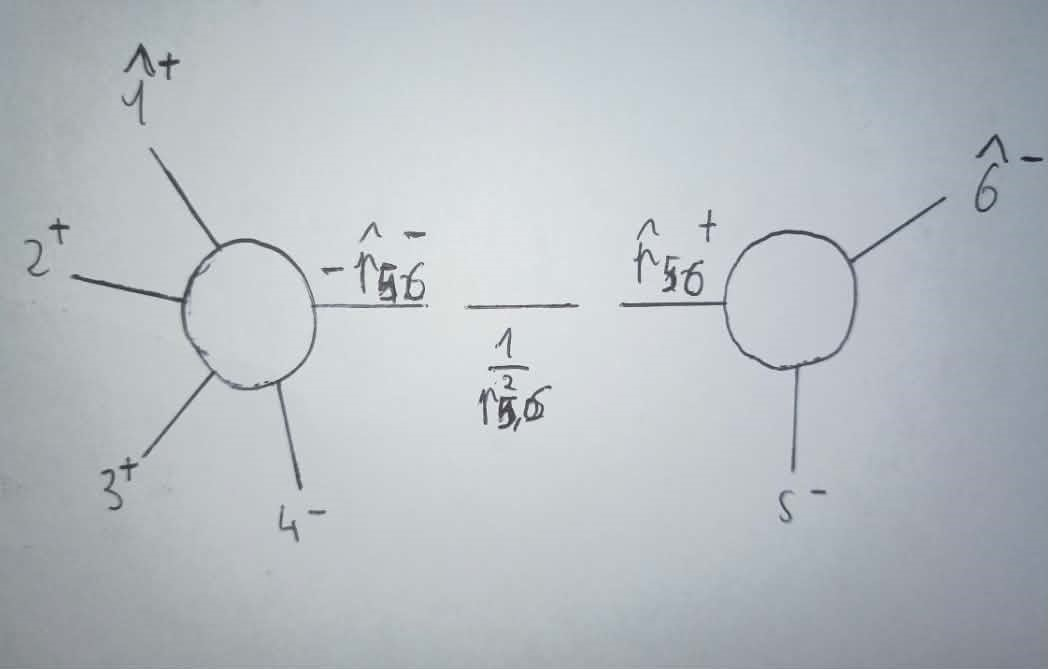
\includegraphics[ width=0.45\textwidth]{diagrammeX} % Don't include .png or .jpg extension
				\label{fig:diagrammeX}
			\end{minipage}		
		\end{figure}
		\begin{figure}[h]
			\centering
			\begin{minipage}[c]{0.10\textwidth}
				\centering
				Pour $\mathbb{Y}$
			\end{minipage}
			\begin{minipage}[c]{0.75\textwidth}	
			\centering
			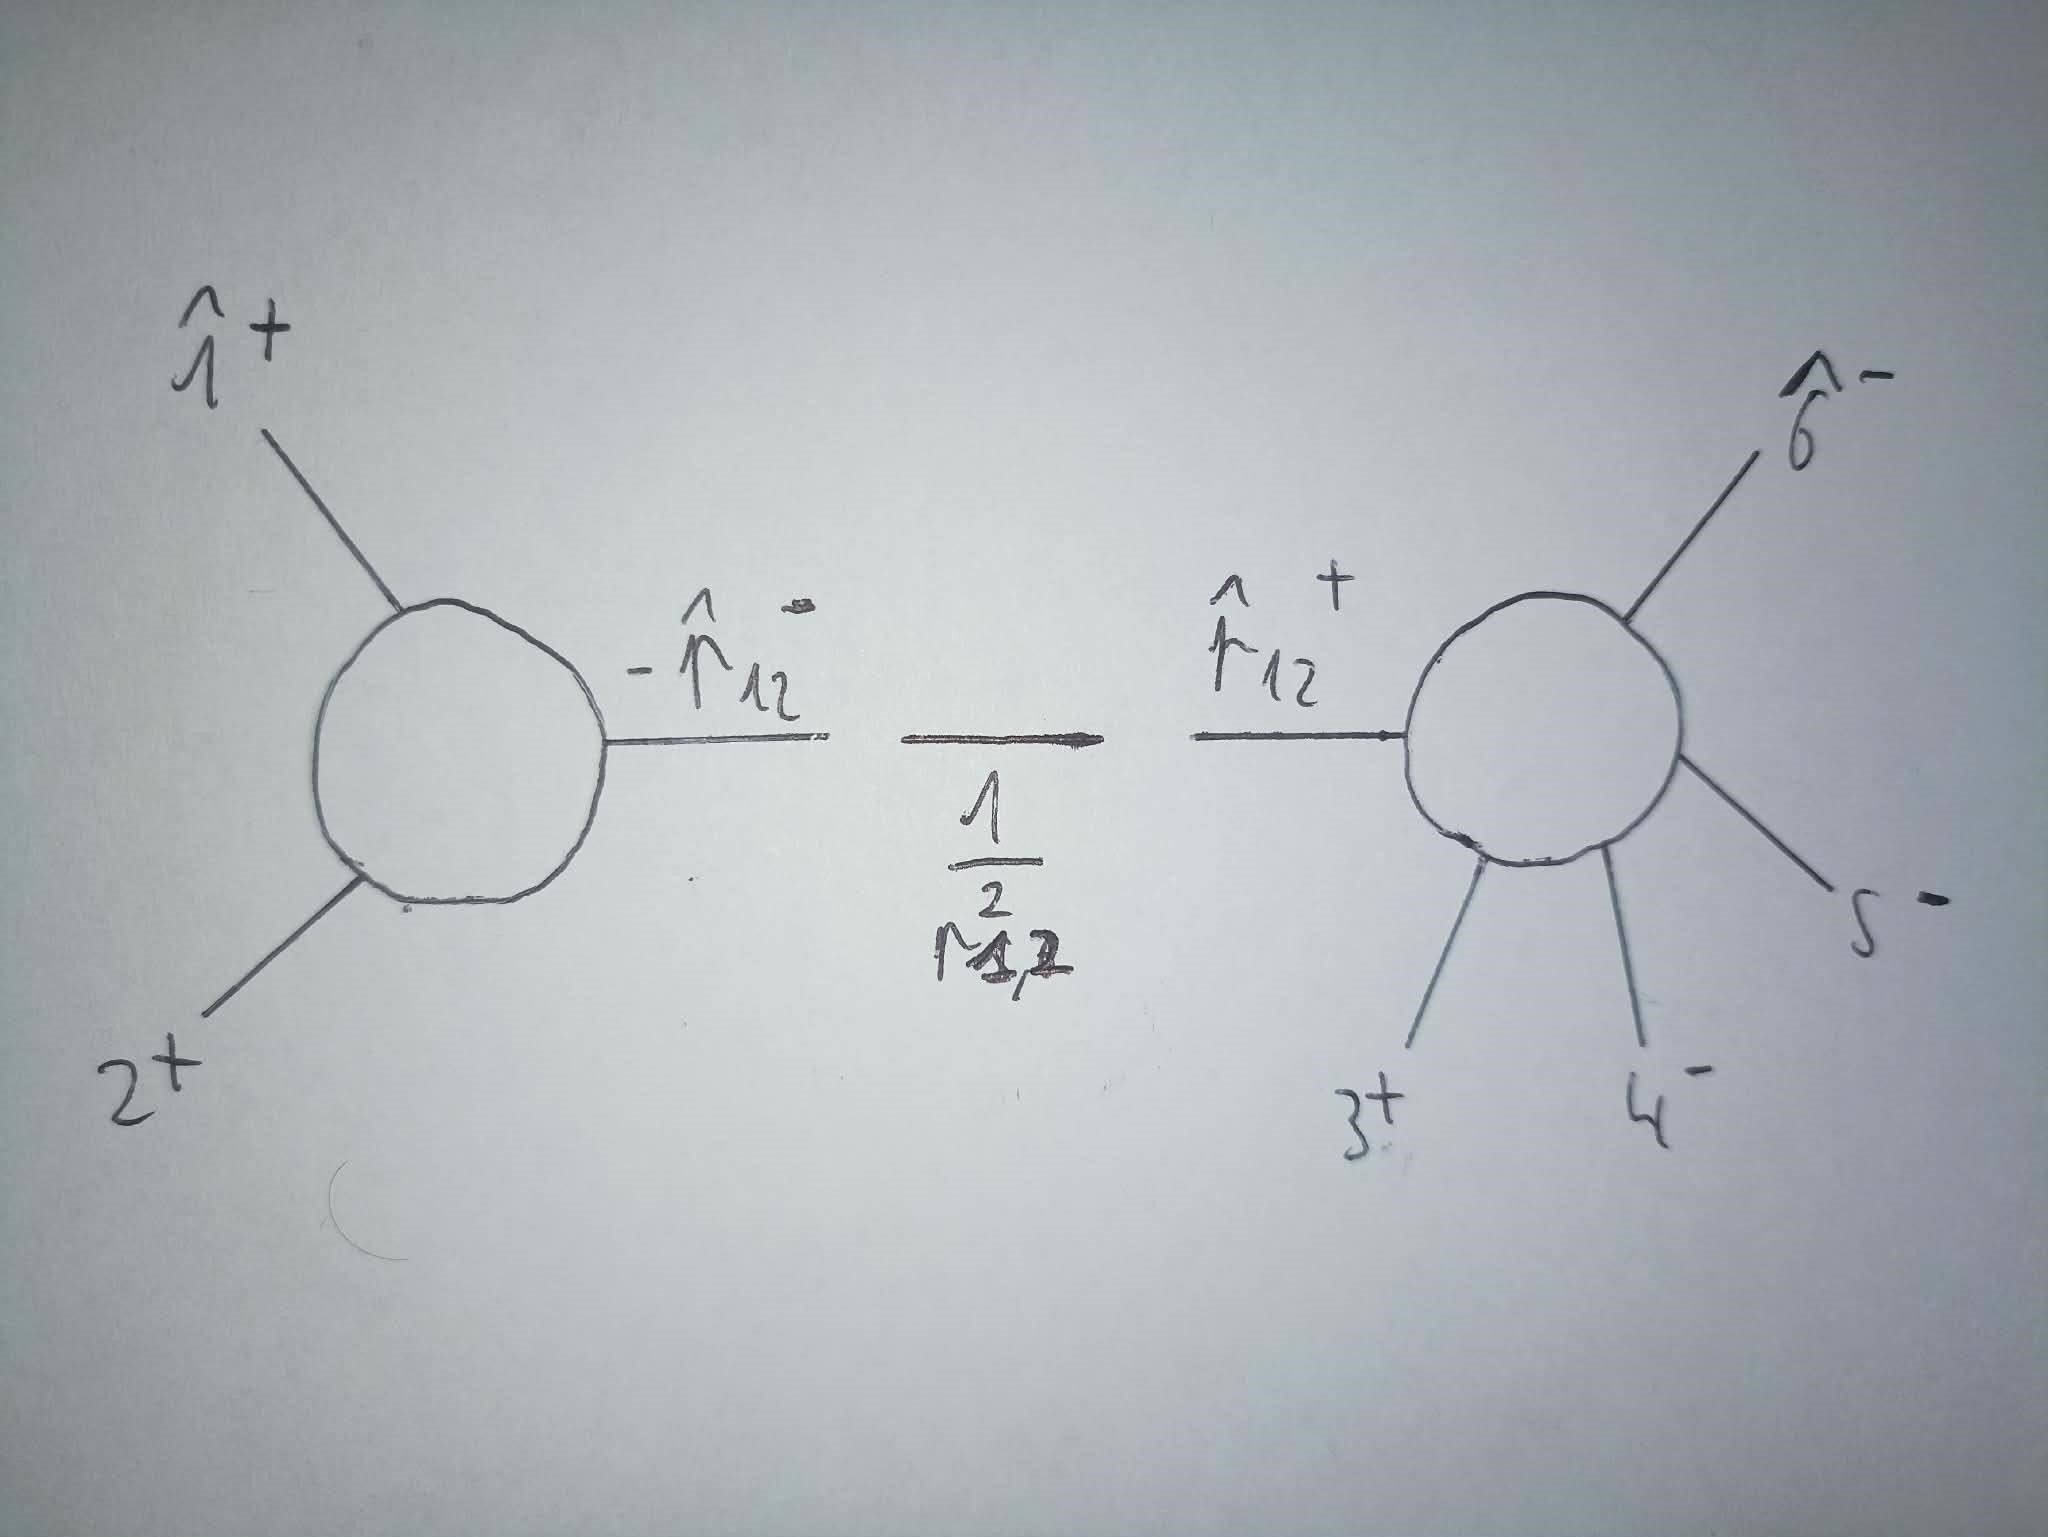
\includegraphics[ width=0.45\textwidth]{diagrammeY} % Don't include .png or .jpg extension
			\label{fig:diagrammeY}
			\end{minipage}		
		\end{figure}
		
		\section{L'amplitude $\mathbb{X}=\mathcal{A}(\hat{1}^+, 2^+, 3^+, 4^-, -\hat{p}_{5,6}^-) \frac{1}{p_{5,6}^2} \mathcal{A}(\hat{p}_{5,6}^+, 5^-, 6^-)$}
		
		Nous partons de:
		\[\mathbb{X}=\mathcal{A}(\hat{1}^+, 2^+, 3^+, 4^-, -\hat{p}_{5,6}^-) \frac{1}{p_{5,6}^2} \mathcal{A}(\hat{p}_{5,6}^+, 5^-, 6^-)\]
		En utilisant la formule de Parke-Taylor et des amplitudes $\mathcal{A}_3$ pour les MHV et en tenant compte du shift que l'on a choisit, cette expression devient:
		\begin{equation}
			\begin{split}
				\mathbb{X}
				&=\frac{(-1)^4 \langle 4 \hat{p}_{5,6} \rangle^4}
				{\langle \hat{1}2 \rangle \langle 23 \rangle \langle 34 \rangle 
				(-1) \langle 4 \hat{p}_{5,6} \rangle (-1) \langle \hat{p}_{5,6}\hat{1} \rangle } \times \frac{1}{p_{5,6}^2} \times \frac{\langle 56 \rangle^4}
				{\langle \hat{p}_{5,6} 5 \rangle \langle 56 \rangle 
				\langle 6\hat{p}_{5,6} \rangle}\\
				&=\frac{\langle 4 \hat{p}_{5,6} \rangle^3}
				{\langle \hat{1}2 \rangle \langle 23 \rangle \langle 34 \rangle 
					\langle \hat{p}_{5,6}\hat{1} \rangle } \times \frac{1}{p_{5,6}^2} \times \frac{\langle 56 \rangle^3}
				{\langle \hat{p}_{5,6} 5 \rangle 
					\langle 6\hat{p}_{5,6} \rangle}\\
				&=\frac{\langle 4 \hat{p}_{5,6} \rangle^3 [\hat{p}_{5,6}1]^3}
				{\langle \hat{1}2 \rangle \langle 23 \rangle \langle 34 \rangle 
					\langle \hat{p}_{5,6}\hat{1} \rangle [\hat{p}_{5,6}1] } \times \frac{1}{p_{5,6}^2} \times \frac{\langle 56 \rangle^3}
				{\langle \hat{p}_{5,6} 5 \rangle[\hat{p}_{5,6}1] 
					\langle 6\hat{p}_{5,6} \rangle[\hat{p}_{5,6}1]}\\
			\end{split}
		\end{equation}
		Il nous faut maintenant calculer certains termes dans cette expression.
		\subsection{}
		\begin{equation}
			\begin{split}
				\langle 4 \hat{p}_{5,6} \rangle [\hat{p}_{5,6}1]
				&=\langle 4(\hat{p}_{5,6})1]\\
				&=\langle 4 (k_5 +\hat{k}_6)1 ]\\
				&=\langle 4 (\lambda_5\bar{\lambda}_5 + \lambda_6 \hat{\bar{\lambda}}_6)1]\\
				&=\langle 4 \lambda_5\bar{\lambda}_5 1] + \langle 4 \lambda_6\hat{\bar{\lambda}}_6 1]\\
				&=\langle 451] +\langle 4\hat{6}1] \\
				&=\langle 451] +\langle 46 \rangle [\hat{6}1] \\
				&=\langle 451] +\langle 46 \rangle ([61]+z[11]) \\
				&=\langle 4(5+6)1]
			\end{split}
		\end{equation}
		
		\subsection{}
		\begin{equation}
			\begin{split}
				\langle \hat{p}_{5,6}\hat{1} \rangle [\hat{p}_{5,6}1]
				&=- \langle \hat{1} \hat{p}_{5,6} \rangle [\hat{p}_{5,6}1]\\
				&=-(\langle \hat{1}5 \rangle [51]+ \langle \hat{1}6 \rangle [\hat{6}1])\\
				&=-(\langle 15 \rangle -z \langle 65 \rangle )[51]-(\langle 16 \rangle -z\langle 66 \rangle)([61]+z[11])\\
				&=-\langle 15 \rangle [51] - \langle 16 \rangle [61] + z \langle 65 \rangle [51]\\
			\end{split}
		\end{equation}
		
		Or, on a:  
		\[k_5 + \hat{k}_6 + \hat{p}_{5,6}=0 \Leftrightarrow \hat{p}_{5,6}=-(k_5 + k_6) \]\\
		
		Ce qui nous donne:
		\[\hat{p}_{5,6}^2=0 \Leftrightarrow 2k_5 \hat{k}_6 = \langle 56 \rangle [\hat{6}5]=0\]\\
		
		En développant, on trouve que: 
		\[\langle 56 \rangle ([65]+z[15])=0 \Leftrightarrow z=-\frac{[65]}{15}=-\frac{[56]}{[51]}=\frac{[65]}{[51]}\]
		
		En injectant cette valeur de z dans la dernière forme de $(5)$, on trouve que:
		\[\langle \hat{p}_{5,6}\hat{1} \rangle [\hat{p}_{5,6}1]= -\langle 15 \rangle [51] - \langle 16 \rangle [61] - \langle 65 \rangle [56] \]\\
		
		Or, on a aussi que:
		\[(k_{5,1})^2=(k_5 + k_6 +k_1)^2 = 2k_5 k_6 + 2k_5 k_1 +2k_6 k_1= \langle 15 \rangle [51] + \langle 16 \rangle [61] + \langle 65 \rangle [56]\]
		
		Ainsi, nous obtenons l'expression:
		\[\langle \hat{p}_{5,6}\hat{1} \rangle [\hat{p}_{5,6}1]= -(k_{5,1})^2 \]
		
		\subsection{}
		\begin{equation}
			\begin{split}
				\langle \hat{p}_{5,6} 5 \rangle[\hat{p}_{5,6}1]
				&=- \langle 5 \hat{p}_{5,6}  \rangle[\hat{p}_{5,6}1]\\
				&=- \langle 55 \rangle [51] - \langle 56 \rangle [\hat{6}1]\\
				&=- \langle 56 \rangle ([61]+z[11])\\
				&=- \langle 56 \rangle [61]
			\end{split}
		\end{equation}
		
		\subsection{}
		\begin{equation}
			\begin{split}
				\langle 6\hat{p}_{5,6} \rangle[\hat{p}_{5,6}1]
				&= \langle 65  \rangle[51] + \langle 66 \rangle [\hat{6}1]\\
				&= \langle 65 \rangle [51]
			\end{split}
		\end{equation}
		
		\subsection{}
		\begin{equation}
			\begin{split}
				p_{5,6}^2
				&= 2 k_5 k_6\\
				&= \langle 56 \rangle [65]
			\end{split}
		\end{equation}
		
		\subsection{}
		\begin{equation}
			\begin{split}
				\langle \hat{1}2 \rangle
				&= \langle 12 \rangle -z \langle 62 \rangle \\
				&= \langle 12 \rangle -\frac{[65]}{[51]} \langle 62 \rangle \\
				&= \frac{\langle 12 \rangle[51]-\langle 62 \rangle[65]}{[51]} \\
				&= \frac{\langle 21 \rangle[15]+\langle 26 \rangle[65]}{[51]} \\
				&= \frac{\langle 2(1+6)5]}{[51]}
			\end{split}
		\end{equation}
		
		\subsection{L'expression finale de l'amplitude $\mathbb{X}$}
		On avait:
		\[\mathbb{X}=\frac{\langle 4 \hat{p}_{5,6} \rangle^3 [\hat{p}_{5,6}1]^3}
		{\langle \hat{1}2 \rangle \langle 23 \rangle \langle 34 \rangle 
			\langle \hat{p}_{5,6}\hat{1} \rangle [\hat{p}_{5,6}1] } \times \frac{1}{p_{5,6}^2} \times \frac{\langle 56 \rangle^3}
		{\langle \hat{p}_{5,6} 5 \rangle[\hat{p}_{5,6}1] 
			\langle 6\hat{p}_{5,6} \rangle[\hat{p}_{5,6}1]}\]
		
		En injectant les expressions trouvées de $3.1$ à $3.6$ dans cette dernière, on trouve:
		
		\begin{equation}
			\begin{split}
				\mathbb{X}
				&=\frac{\langle 4(5+6)1]^3 \langle 56 \rangle^3}{\frac{\langle 2(1+6)5]}{[51]} \langle 23 \rangle \langle 34 \rangle (-(k_{5,1})^2)\langle 56 \rangle [65]
				(-1)\langle 56 \rangle [61]\langle 65 \rangle [51]}\\
				&=\frac{\langle 4(5+6)1]^3 \langle 56 \rangle^3}{\frac{\langle 2(1+6)5]}{[51]} \langle 23 \rangle \langle 34 \rangle (-(k_{5,1})^2)\langle 56 \rangle (-1)[56]
				(-1)\langle 56 \rangle [61](-1)\langle 56 \rangle [51]}\\
				\mathbb{X}&=\frac{\langle 4(5+6)1]^3 }{(k_{5,1})^2  \langle 23 \rangle \langle 34 \rangle [56][61]\langle 2(1+6)5]}
			\end{split}
		\end{equation}		
		
		\section{L'amplitude $\mathbb{Y}=\mathcal{A}(\hat{1}^+, 2^+, -\hat{p}_{1,2}^-) \frac{1}{p_{1,2}^2} \mathcal{A}(\hat{p}_{1,2}^+, 3^+, 4^-, 5^-, 6^-)$}
		
		Nous partons cette fois de l'expression suivante:
		
		\[\mathbb{Y}=\mathcal{A}(\hat{1}^+, 2^+, -\hat{p}_{1,2}^-) \frac{1}{p_{1,2}^2} \mathcal{A}(\hat{p}_{1,2}^+, 3^+, 4^-, 5^-, 6^-)\]
		
		En utilisant cette fois-ci les formules de Parke-Taylor et $\mathcal{A}$ pour les amplitudes anti-MHV, on trouve que:
		
		\begin{equation}
			\begin{split}
				\mathbb{Y}
				&=\frac{[12]^4}{[12](-1)[2\hat{p}_{1,2}](-1)[\hat{p}_{1,2}1]} 
				\times \frac{1}{p_{1,2}^2} \times
				\frac{[\hat{p}_{1,2}3]^4}{[\hat{p}_{1,2}3][34][45][5\hat{6}][\hat{6}\hat{p}_{1,2}]} \\
				&=\frac{[12]^3}{[2\hat{p}_{1,2}][\hat{p}_{1,2}1]} 
				\times \frac{1}{p_{1,2}^2} \times
				\frac{[\hat{p}_{1,2}3]^3}{[34][45][5\hat{6}][\hat{6}\hat{p}_{1,2}]} \\
				&=\frac{[12]^3}{\langle 6 \hat{p}_{1,2} \rangle[2\hat{p}_{1,2}]\langle 6 \hat{p}_{1,2} \rangle[\hat{p}_{1,2}1]} 
				\times \frac{1}{p_{1,2}^2} \times
				\frac{\langle 6 \hat{p}_{1,2} \rangle^3 [\hat{p}_{1,2}3]^3}{[34][45][5\hat{6}]\langle 6 \hat{p}_{1,2} \rangle[\hat{6}\hat{p}_{1,2}]} \\
			\end{split}
		\end{equation}
		
		Nous allons maintenant calculer les termes petit à petit pour simplifier cette expression
		
		\subsection{}
		\begin{equation}
			\begin{split}
				\langle 6 \hat{p}_{1,2} \rangle [\hat{p}_{1,2}3]
				&=\langle 6 \hat{1} \rangle [13] + \langle 62 \rangle [23]\\
				&=(\langle 61 \rangle -z \langle 66 \rangle)[13]+ \langle 62 \rangle [23]\\
				&=\langle 61 \rangle [13] + \langle 62 \rangle [23]\\
				&=\langle 6(1+2)3] \\
			\end{split}
		\end{equation}
		
		\subsection{}
		\begin{equation}
			\begin{split}
				\langle 6 \hat{p}_{1,2} \rangle [2\hat{p}_{1,2}]
				&=-\langle 6 \hat{p}_{1,2} \rangle [\hat{p}_{1,2}2]\\
				&=-(\langle 6 \hat{1} \rangle[12] + \langle 62 \rangle [22])\\
				&=(\langle 61 \rangle - z \langle 66 \rangle)[12]\\
				&=- \langle 61 \rangle [12]
			\end{split}
		\end{equation}
		
		\subsection{}
		\begin{equation}
			\begin{split}
				\langle 6 \hat{p}_{1,2} \rangle [\hat{p}_{1,2}1]
				&=\langle 6 \hat{1} \rangle [11] + \langle 62 \rangle [21] \\
				&=\langle 62 \rangle [21]
			\end{split}
		\end{equation}
		
		\subsection{}
		\begin{equation}
			\begin{split}
				\langle 6 \hat{p}_{1,2} \rangle [\hat{6}\hat{p}_{1,2}]
				&=-\langle 6 \hat{p}_{1,2} \rangle [\hat{p}_{1,2}\hat{6}] \\
				&=-(\langle 6 \hat{1} \rangle [1 \hat{6}] + \langle 62 \rangle [2 \hat{6}])\\
				&=- (\langle 61 \rangle - z \langle 66 \rangle)([16] + z [11]) 
				- \langle 62 \rangle ([26] + z [21])\\
				&= - \langle 61 \rangle [16] - \langle 62 \rangle [26] 
				- z \langle 62 \rangle [21]
			\end{split}
		\end{equation}
		
		Or, nous savons que : $-\hat{p}_{1,2} + \hat{k}_1 + k_2 =0 \Leftrightarrow \hat{p}_{1,2} =\hat{k}_1 + k_2  $\\
		
		Ainsi : $ (\hat{p}_{1,2})^2= 2 \hat{k}_1 k_2 = \langle \hat{1} 2 \rangle [21] =0 $ \\
		
		Ce qui nous donne en développant le shift: $(\langle 12 \rangle - z \langle 62 \rangle)[21]=0 \Leftrightarrow \langle 12 \rangle - z \langle 62 \rangle =0 \Leftrightarrow z= \frac{\langle 12 \rangle}{\langle 62 \rangle}$
		
		En injectant dans (15), on trouve que:
		\[\langle 6 \hat{p}_{1,2} \rangle [\hat{6}\hat{p}_{1,2}]=
		- \langle 61 \rangle [16] - \langle 62 \rangle [26] 
		- \langle 12 \rangle [21]\]
		
		Or, nous avons aussi :
		\begin{equation}
			\begin{split}
				k_{6,2}= k_6 + k_1 + k_2 \Rightarrow (k_{6,2})^2
				&= 2k_6 k_1 + 2k_1 k_2 + 2k_6 k_2 \\
				&=	\langle 61 \rangle [16] + \langle 62 \rangle [26] 
				+\langle 12 \rangle [21]
			\end{split}
		\end{equation}
		
		Par conséquent, nous pouvons faire l'identification suivante:
		
		\[\langle 6 \hat{p}_{1,2} \rangle [\hat{6}\hat{p}_{1,2}]=-(k_{6,2})^2\]
		
		\subsection{}
		\begin{equation}
			\begin{split}
				(p_{1,2})^2
				&=(k_1 + k_2)^2\\
				&=2k_1 k_2\\
				&=\langle 12 \rangle [21]
			\end{split}
		\end{equation}
		
		\subsection{}
		\begin{equation}
			\begin{split}
				[5\hat{6}]
				&=[56] + z[51] \\
				&=[56] + \frac{\langle 12 \rangle}{\langle 62 \rangle}[51] \\
				&=\frac{[56]\langle 62 \rangle +\langle 12 \rangle [51]} {\langle 62 \rangle}\\
				&=\frac{\langle 26 \rangle[65] +\langle 21 \rangle [15]} {\langle 62 \rangle}\\
				&=\frac{\langle 2 (1+6) 5]}{\langle 62 \rangle}
			\end{split}
		\end{equation}
		
		\subsection{L'expression finale de l'amplitude $\mathbb{Y}$}
		On avait:
		
		\[\mathbb{Y}=\frac{[12]^3}{\langle 6 \hat{p}_{1,2} \rangle[2\hat{p}_{1,2}]\langle 6 \hat{p}_{1,2} \rangle[\hat{p}_{1,2}1]} 
		\times \frac{1}{p_{1,2}^2} \times
		\frac{\langle 6 \hat{p}_{1,2} \rangle^3 [\hat{p}_{1,2}3]^3}{[34][45][5\hat{6}]\langle 6 \hat{p}_{1,2} \rangle[\hat{6}\hat{p}_{1,2}]}\]
		
		En injectant les expressions trouvées de $4.1$ à $4.6$ dans cette dernière, on trouve que:
		
		\begin{equation}
			\begin{split}
				\mathbb{Y}
				&=\frac{[12]^3}{(-1) \langle 61 \rangle [12]\langle 62 \rangle [21]} 
				\times \frac{1}{\langle 12 \rangle [21]} \times
				\frac{\langle 6(1+2)3]^3}{[34][45]\frac{\langle 2 (1+6) 5]}{\langle 62 \rangle}(-1)(k_{6,2})^2}\\
				&=\frac{[12]^3}{(-1) \langle 61 \rangle [12]\langle 62 \rangle (-1)[12]} 
				\times \frac{1}{\langle 12 \rangle (-1)[12]} \times
				\frac{\langle 6(1+2)3]^3}{[34][45]\frac{\langle 2 (1+6) 5]}{\langle 62 \rangle}(-1)(k_{6,2})^2}\\
				\mathbb{Y}&=\frac{\langle 6(1+2)3]^3}{(k_{6,2})^2 \langle 61 \rangle \langle 12 \rangle [34][45]\langle 2 (1+6) 5]}
			\end{split}
		\end{equation}
		
		\section{L'amplitude totale $\mathcal{A}(1^+, 2^+, 3^+, 4^-, 5^-, 6^-)$}
		
		On a : 
		\[\mathcal{A}(1^+, 2^+, 3^+, 4^-, 5^-, 6^-)=\mathbb{X} + \mathbb{Y}\]
		
		Et on a :
		\begin{equation}
			\begin{split}
				\mathbb{X}
				&=\frac{\langle 4(5+6)1]^3 }{(k_{5,1})^2  \langle 23 \rangle \langle 34 \rangle [56][61]\langle 2(1+6)5]}\\
				\mathbb{Y}
				&=\frac{\langle 6(1+2)3]^3}{(k_{6,2})^2 \langle 61 \rangle \langle 12 \rangle [34][45]\langle 2 (1+6) 5]}
			\end{split}
		\end{equation}
		
		Et en faisant la somme, on trouve finalement que:
		\[\mathcal{A}(1^+, 2^+, 3^+, 4^-, 5^-, 6^-)=
		\frac{\langle 4(5+6)1]^3 }{(k_{5,1})^2  \langle 23 \rangle \langle 34 \rangle [56][61]\langle 2(1+6)5]}
		+
		\frac{\langle 6(1+2)3]^3}{(k_{6,2})^2 \langle 61 \rangle \langle 12 \rangle [34][45]\langle 2 (1+6) 5]}\]
		
		
		
\end{document}